\documentclass[10pt]{article}
\usepackage[utf8]{inputenc}
\usepackage[T1]{fontenc}
\usepackage{amsmath}
\usepackage{amsfonts}
\usepackage{amssymb}
\usepackage[version=4]{mhchem}
\usepackage{stmaryrd}
\usepackage{hyperref}
\usepackage{graphicx}
\usepackage{enumitem}
\usepackage{multirow}
\usepackage{amsthm}
\usepackage{parskip}
\graphicspath{ {./CS-234/} }

\title{Assignment 6 - Inductive Proofs}

\author{CS 234}
\date{Daniel Lee}


\begin{document}
\maketitle

\section*{1 \quad Last 2 Proofs on Paper}

\begin{enumerate}[label={}]
      \item Draw DFAs with as few states as possible for each of the following languages and then prove that they accept that language.\\

            9.3 $\left\{w \in\{0,1\}^*: w\right.$ has 01 as a substring $\}$\\
            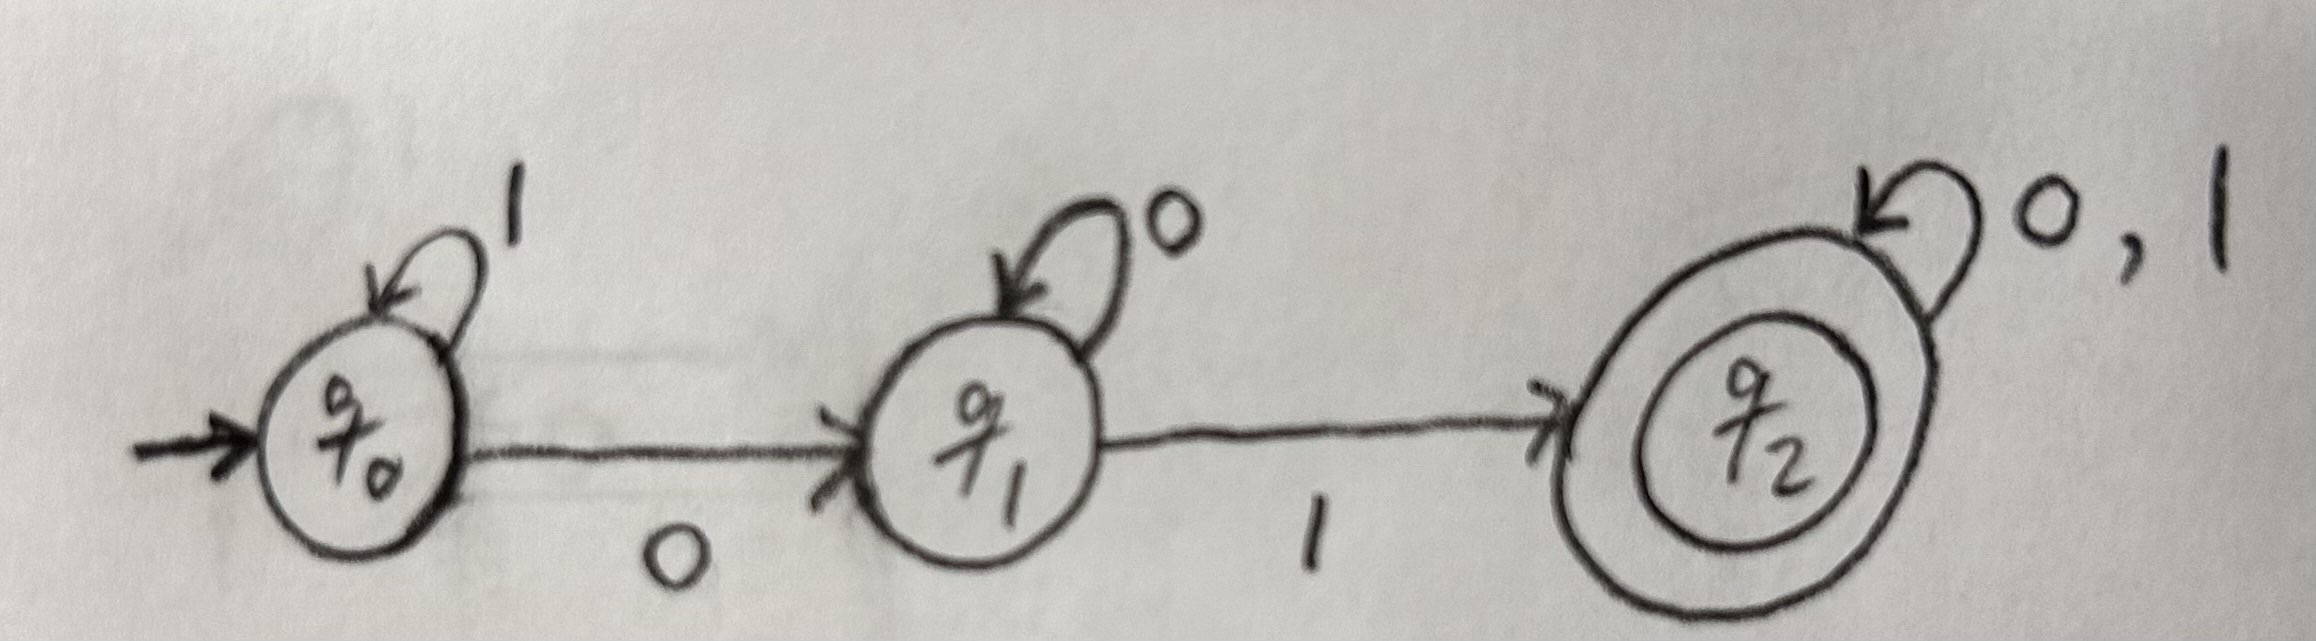
\includegraphics[scale=0.1]{9.3}
            \begin{proof}
                  This statement is proven by mutual induction using the following 3 predicates:\\
                  $$
                        \begin{aligned}
                               & A(n):=\forall w \in\{0,1\}^* .|w|=n \rightarrow\left(\hat{\delta}\left(q_0, w\right)=q_0 \leftrightarrow w \text { doesn't have 01 as a substring} \right. \\
                               & \quad \left. \text{and doesn't end with } 0\right)                                                                                                         \\
                               & B(n):=\forall w \in\{0,1\}^* .|w|=n \rightarrow\left(\hat{\delta}\left(q_0, w\right)=q_1 \leftrightarrow w \text { doesn't have 01 as a substring} \right. \\
                               & \quad \left. \text{and ends with } 0\right)                                                                                                                \\
                               & C(n):=\forall w \in\{0,1\}^* .|w|=n \rightarrow\left(\hat{\delta}\left(q_0, w\right)=q_2 \leftrightarrow w \text { has 01 as a substring }\right)
                        \end{aligned}
                  $$

                  \textbf{Base case} $n=0$: Let $w$ be an arbitrary string over the alphabet $\{0,1\}$ that is of length 0. Then we know that $w=\lambda$ and $\hat{\delta}\left(q_0, w\right)=\hat{\delta}\left(q_0, \lambda\right)$. By definition of $\hat{\delta}$, we find that $\hat{\delta}\left(q_0, \lambda\right)=q_0$.\\
                  Thus, both sides of $A(0)$'s biconditional are satisfied, rendering $A(0)$ true.\\
                  At the same time, since $q_0 \neq q_1, q_0 \neq q_2, \lambda$ does not end with 0, and $\lambda$ does not have 01 as a substring, both sides of $B(0)$'s biconditional are false and both sides of $C(0)$'s biconditional are false, rendering $B(0)$ and $C(0)$ true.\\

                  \textbf{Inductive case :} Suppose for the inductive hypothesis that all of $A(n), B(n)$, and $C(n)$ hold for some natural $n$. We want to show each of $A(n+1), B(n+1)$, and $C(n+1)$.\\
                  Let $w$ be an arbitrary string over the alphabet $\{0,1\}$ of length $n+1$. Because $n+1 \geq 1$, it must be that $w=v c$ for some string $v \in\{0,1\}^*$ of length $n$ and $c \in\{0,1\}$.\\
                  The proof now proceeds by cases over the result of $\hat{\delta}\left(q_0, v\right)$ and the identity of $c$.\\

                  \textbf{Subcase }$\hat{\delta}\left(q_0, v\right)=q_0$ and $c=0$: Suppose that $\hat{\delta}\left(q_0, v\right)=q_0$ and $c=0$. Observe then the following:
                  $$
                        \begin{aligned}
                              \hat{\delta}\left(q_0, w\right) & =\hat{\delta}\left(q_0, v 0\right)                     & {[w=v c, c=0] }                                     \\
                                                              & =\delta\left(\hat{\delta}\left(q_0, v\right), 0\right) & {[\hat{\delta} \text { def}] }                      \\
                                                              & =\delta\left(q_0, 0\right)                             & {\left[\hat{\delta}\left(q_0, v\right)=q_0\right] } \\
                                                              & =q_1                                                   & {[\delta \operatorname{def}] . }
                        \end{aligned}
                  $$
                  Further, because $\hat{\delta}\left(q_0, v\right)=q_0$, the inductive hypothesis tells us that $v$ does not have 01 as a substring and does not end with 0. Thus, we know that $w=v0$ does not have 01 as a substring and ends with 0.\\
                  This leaves both sides of $B(n+1)$'s biconditional true, rendering $B(n+1)$ true.\\
                  At the same time, because $\hat{\delta}\left(q_0, w\right)$ is not $q_0$ or $q_2$ and $w$ does not have 01 as a substring and ends with 0, both sides of $A(n+1)$ and $C(n+1)$'s biconditionals are false, rendering both $A(n+1)$ and $C(n+1)$ true.\\

                  \textbf{Subcase }$\hat{\delta}\left(q_0, v\right)=q_0$ and $c=1$: Suppose that $\hat{\delta}\left(q_0, v\right)=q_0$ and $c=1$. Observe then the following:
                  $$
                        \begin{aligned}
                              \hat{\delta}\left(q_0, w\right) & =\hat{\delta}\left(q_0, v 1\right)                     & {[w=v c, c=1] }                                     \\
                                                              & =\delta\left(\hat{\delta}\left(q_0, v\right), 1\right) & {[\hat{\delta} \text { def}] }                      \\
                                                              & =\delta\left(q_0, 1\right)                             & {\left[\hat{\delta}\left(q_0, v\right)=q_0\right] } \\
                                                              & =q_0                                                   & {[\delta \operatorname{def}] . }
                        \end{aligned}
                  $$
                  Further, because $\hat{\delta}\left(q_0, v\right)=q_0$, the inductive hypothesis tells us that $v$ does not have 01 as a substring and does not end with 0. Thus, we know that $w=v1$ does not have 01 as a substring and doesn't end with 0.\\
                  This leaves both sides of $A(n+1)$'s biconditional true, rendering $A(n+1)$ true.\\
                  At the same time, because $\hat{\delta}\left(q_0, w\right)$ is not $q_1$ or $q_2$ and $w$ does not have 01 as a substring and doesn't end with 0, both sides of $B(n+1)$ and $C(n+1)$'s biconditionals are false, rendering both $B(n+1)$ and $C(n+1)$ true.\\

                  \textbf{Subcase }$\hat{\delta}\left(q_0, v\right)=q_1$ and $c=0$: Suppose that $\hat{\delta}\left(q_0, v\right)=q_1$ and $c=0$. Observe then the following:
                  $$
                        \begin{aligned}
                              \hat{\delta}\left(q_0, w\right) & =\hat{\delta}\left(q_0, v 0\right)                     & {[w=v c, c=0] }                                     \\
                                                              & =\delta\left(\hat{\delta}\left(q_0, v\right), 0\right) & {[\hat{\delta} \text { def}] }                      \\
                                                              & =\delta\left(q_1, 0\right)                             & {\left[\hat{\delta}\left(q_0, v\right)=q_1\right] } \\
                                                              & =q_1                                                   & {[\delta \operatorname{def}] . }
                        \end{aligned}
                  $$
                  Further, because $\hat{\delta}\left(q_0, v\right)=q_1$, the inductive hypothesis tells us that $v$ does not have 01 as a substring and ends with 0. Thus, we know that $w=v0$ does not have 01 as a substring and ends with 0.\\
                  This leaves both sides of $B(n+1)$'s biconditional true, rendering $B(n+1)$ true.\\
                  At the same time, because $\hat{\delta}\left(q_0, w\right)$ is not $q_0$ or $q_2$ and $w$ does not have 01 as a substring and ends with 0, both sides of $A(n+1)$ and $C(n+1)$'s biconditionals are false, rendering both $A(n+1)$ and $C(n+1)$ true.\\

                  \textbf{Subcase }$\hat{\delta}\left(q_0, v\right)=q_1$ and $c=1$: Suppose that $\hat{\delta}\left(q_0, v\right)=q_1$ and $c=1$. Observe then the following:
                  $$
                        \begin{aligned}
                              \hat{\delta}\left(q_0, w\right) & =\hat{\delta}\left(q_0, v 1\right)                     & {[w=v c, c=1] }                                     \\
                                                              & =\delta\left(\hat{\delta}\left(q_0, v\right), 1\right) & {[\hat{\delta} \text { def}] }                      \\
                                                              & =\delta\left(q_1, 1\right)                             & {\left[\hat{\delta}\left(q_0, v\right)=q_1\right] } \\
                                                              & =q_2                                                   & {[\delta \operatorname{def}] . }
                        \end{aligned}
                  $$
                  Further, because $\hat{\delta}\left(q_0, v\right)=q_1$, the inductive hypothesis tells us that $v$ does not have 01 as a substring and ends with 0. Thus, we know that $w=v1$ has 01 as a substring.\\
                  This leaves both sides of $C(n+1)$'s biconditional true, rendering $C(n+1)$ true.\\
                  At the same time, because $\hat{\delta}\left(q_0, w\right)$ is not $q_0$ or $q_1$ and $w$ has 01 as a substring, both sides of $A(n+1)$ and $B(n+1)$'s biconditionals are false, rendering both $A(n+1)$ and $B(n+1)$ true.\\

                  \textbf{Subcase }$\hat{\delta}\left(q_0, v\right)=q_2$ and $c=0$: Suppose that $\hat{\delta}\left(q_0, v\right)=q_2$ and $c=0$. Observe then the following:
                  $$
                        \begin{aligned}
                              \hat{\delta}\left(q_0, w\right) & =\hat{\delta}\left(q_0, v 0\right)                     & {[w=v c, c=0] }                                     \\
                                                              & =\delta\left(\hat{\delta}\left(q_0, v\right), 0\right) & {[\hat{\delta} \text { def}] }                      \\
                                                              & =\delta\left(q_2, 0\right)                             & {\left[\hat{\delta}\left(q_0, v\right)=q_2\right] } \\
                                                              & =q_2                                                   & {[\delta \operatorname{def}] . }
                        \end{aligned}
                  $$
                  Further, because $\hat{\delta}\left(q_0, v\right)=q_2$, the inductive hypothesis tells us that $v$ has 01 as a substring. Thus, we know that $w=v0$ has 01 as a substring.\\
                  This leaves both sides of $C(n+1)$'s biconditional true, rendering $C(n+1)$ true.\\
                  At the same time, because $\hat{\delta}\left(q_0, w\right)$ is not $q_0$ or $q_1$ and $w$ has 01 as a substring, both sides of $A(n+1)$ and $B(n+1)$'s biconditionals are false, rendering both $A(n+1)$ and $B(n+1)$ true.\\

                  \textbf{Subcase }$\hat{\delta}\left(q_0, v\right)=q_2$ and $c=1$: Suppose that $\hat{\delta}\left(q_0, v\right)=q_2$ and $c=1$. Observe then the following:
                  $$
                        \begin{aligned}
                              \hat{\delta}\left(q_0, w\right) & =\hat{\delta}\left(q_0, v 1\right)                     & {[w=v c, c=1] }                                     \\
                                                              & =\delta\left(\hat{\delta}\left(q_0, v\right), 1\right) & {[\hat{\delta} \text { def}] }                      \\
                                                              & =\delta\left(q_2, 1\right)                             & {\left[\hat{\delta}\left(q_0, v\right)=q_2\right] } \\
                                                              & =q_2                                                   & {[\delta \operatorname{def}] . }
                        \end{aligned}
                  $$
                  Further, because $\hat{\delta}\left(q_0, v\right)=q_2$, the inductive hypothesis tells us that $v$ has 01 as a substring. Thus, we know that $w=v1$ has 01 as a substring.\\
                  This leaves both sides of $C(n+1)$'s biconditional true, rendering $C(n+1)$ true.\\
                  At the same time, because $\hat{\delta}\left(q_0, w\right)$ is not $q_0$ or $q_1$ and $w$ has 01 as a substring, both sides of $A(n+1)$ and $B(n+1)$'s biconditionals are false, rendering both $A(n+1)$ and $B(n+1)$ true.\\
                  \textbf{Conclusion :} Thus, by mutual induction, $A(n)$, $B(n)$, and $C(n)$ hold for all naturals $n$.\\
                  Now observe that the following identities hold for the language of the automaton $M$:
                  $$
                        \begin{aligned}
                              \mathcal{L}(M) & =\left\{w \in\{0, 1\}^* \mid \hat{\delta}(q_0, w) \in\{q_2\}\right\}   &  & {[\mathcal{L} \text { def }] } \\
                                             & =\left\{w \in\{0, 1\}^* \mid \hat{\delta}(q_0, w)=q_2\right\}          &  & {[\text { logic }] }           \\
                                             & =\left\{w \in\{0, 1\}^* \mid w \text { has 01 as a substring }\right\} &  & {[C(|w|)] }
                        \end{aligned}
                  $$

                  This confirms the desired identity for the language of $M$.

            \end{proof}

            \newpage

            9.12 $\left\{w \in\{0,1\}^*: w\right.$ has exactly one 0$\}$\\
            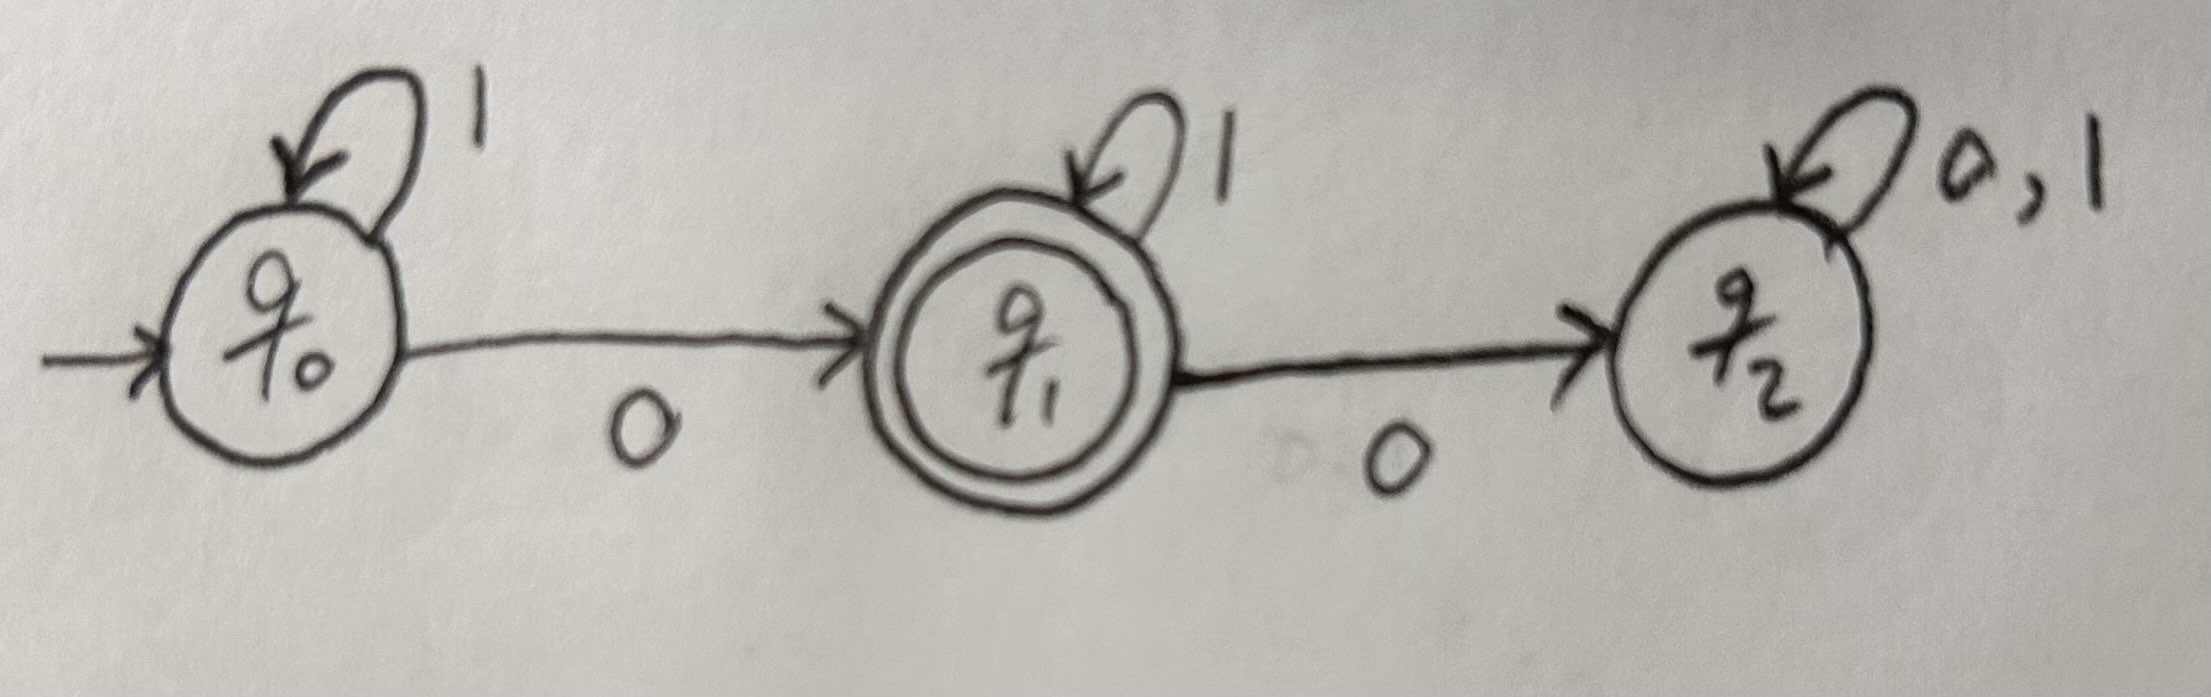
\includegraphics[scale=0.1]{9.12}
            \begin{proof}
                  This statement is proven by mutual induction using the following 3 predicates:\\
                  $$
                        \begin{aligned}
                               & A(n):=\forall w \in\{0,1\}^* .|w|=n \rightarrow\left(\hat{\delta}\left(q_0, w\right)=q_0 \leftrightarrow w \text { has no } 0\right)            \\
                               & B(n):=\forall w \in\{0,1\}^* .|w|=n \rightarrow\left(\hat{\delta}\left(q_0, w\right)=q_1 \leftrightarrow w \text { has exactly one } 0\right)   \\
                               & C(n):=\forall w \in\{0,1\}^* .|w|=n \rightarrow\left(\hat{\delta}\left(q_0, w\right)=q_2 \leftrightarrow w \text { has at least two 0s }\right)
                        \end{aligned}
                  $$

                  \textbf{Base case} $n=0$: Let $w$ be an arbitrary string over the alphabet $\{0,1\}$ that is of length 0. Then we know that $w=\lambda$ and $\hat{\delta}\left(q_0, w\right)=\hat{\delta}\left(q_0, \lambda\right)$. By definition of $\hat{\delta}$, we find that $\hat{\delta}\left(q_0, \lambda\right)=q_0$.\\
                  Thus, both sides of $A(0)$'s biconditional are satisfied, rendering $A(0)$ true.\\
                  At the same time, since $q_0 \neq q_1, q_0 \neq q_2, \lambda$ does not have exactly one 0, and $\lambda$ does not have at least two 0s, both sides of $B(0)$'s biconditional are false and both sides of $C(0)$'s biconditional are false, rendering $B(0)$ and $C(0)$ true.\\

                  \textbf{Inductive case :} Suppose for the inductive hypothesis that all of $A(n), B(n)$, and $C(n)$ hold for some natural $n$. We want to show each of $A(n+1), B(n+1)$, and $C(n+1)$.\\
                  Let $w$ be an arbitrary string over the alphabet $\{0,1\}$ of length $n+1$. Because $n+1 \geq 1$, it must be that $w=v c$ for some string $v \in\{0,1\}^*$ of length $n$ and $c \in\{0,1\}$.\\
                  The proof now proceeds by cases over the result of $\hat{\delta}\left(q_0, v\right)$ and the identity of $c$.\\

                  \textbf{Subcase }$\hat{\delta}\left(q_0, v\right)=q_0$ and $c=0$: Suppose that $\hat{\delta}\left(q_0, v\right)=q_0$ and $c=0$. Observe then the following:
                  $$
                        \begin{aligned}
                              \hat{\delta}\left(q_0, w\right) & =\hat{\delta}\left(q_0, v 0\right)                     & {[w=v c, c=0] }                                     \\
                                                              & =\delta\left(\hat{\delta}\left(q_0, v\right), 0\right) & {[\hat{\delta} \text { def}] }                      \\
                                                              & =\delta\left(q_0, 0\right)                             & {\left[\hat{\delta}\left(q_0, v\right)=q_0\right] } \\
                                                              & =q_1                                                   & {[\delta \operatorname{def}] . }
                        \end{aligned}
                  $$
                  Further, because $\hat{\delta}\left(q_0, v\right)=q_0$, the inductive hypothesis tells us that $v$ has no 0. Thus, we know that $w=v0$ has exactly one 0.\\
                  This leaves both sides of $B(n+1)$'s biconditional true, rendering $B(n+1)$ true.\\
                  At the same time, because $\hat{\delta}\left(q_0, w\right)$ is not $q_0$ or $q_2$ and $w$ has exactly one 0, both sides of $A(n+1)$ and $C(n+1)$'s biconditionals are false, rendering both $A(n+1)$ and $C(n+1)$ true.\\

                  \textbf{Subcase }$\hat{\delta}\left(q_0, v\right)=q_0$ and $c=1$: Suppose that $\hat{\delta}\left(q_0, v\right)=q_0$ and $c=1$. Observe then the following:
                  $$
                        \begin{aligned}
                              \hat{\delta}\left(q_0, w\right) & =\hat{\delta}\left(q_0, v 1\right)                     & {[w=v c, c=1] }                                     \\
                                                              & =\delta\left(\hat{\delta}\left(q_0, v\right), 1\right) & {[\hat{\delta} \text { def}] }                      \\
                                                              & =\delta\left(q_0, 1\right)                             & {\left[\hat{\delta}\left(q_0, v\right)=q_0\right] } \\
                                                              & =q_0                                                   & {[\delta \operatorname{def}] . }
                        \end{aligned}
                  $$
                  Further, because $\hat{\delta}\left(q_0, v\right)=q_0$, the inductive hypothesis tells us that $v$ has no 0. Thus, we know that $w=v1$ has no 0.\\
                  This leaves both sides of $A(n+1)$'s biconditional true, rendering $A(n+1)$ true.\\
                  At the same time, because $\hat{\delta}\left(q_0, w\right)$ is not $q_1$ or $q_2$ and $w$ has no 0, both sides of $B(n+1)$ and $C(n+1)$'s biconditionals are false, rendering both $B(n+1)$ and $C(n+1)$ true.\\

                  \textbf{Subcase }$\hat{\delta}\left(q_0, v\right)=q_1$ and $c=0$: Suppose that $\hat{\delta}\left(q_0, v\right)=q_1$ and $c=0$. Observe then the following:
                  $$
                        \begin{aligned}
                              \hat{\delta}\left(q_0, w\right) & =\hat{\delta}\left(q_0, v 0\right)                    & {[w=v c, c=0] }                                     \\
                                                              & =\delta\left(\hat{\delta}\left(q_0, v\right),0\right) & {[\hat{\delta} \text { def}] }                      \\
                                                              & =\delta\left(q_1, 0\right)                            & {\left[\hat{\delta}\left(q_0, v\right)=q_1\right] } \\
                                                              & =q_2                                                  & {[\delta \operatorname{def}] . }
                        \end{aligned}
                  $$
                  Further, because $\hat{\delta}\left(q_0, v\right)=q_1$, the inductive hypothesis tells us that $v$ has exactly one 0. Thus, we know that $w=v0$ has at least two 0s.\\
                  This leaves both sides of $C(n+1)$'s biconditional true, rendering $C(n+1)$ true.\\
                  At the same time, because $\hat{\delta}\left(q_0, w\right)$ is not $q_0$ or $q_1$ and $w$ has at least two 0s, both sides of $A(n+1)$ and $B(n+1)$'s biconditionals are false, rendering both $A(n+1)$ and $B(n+1)$ true.\\

                  \textbf{Subcase }$\hat{\delta}\left(q_0, v\right)=q_1$ and $c=1$: Suppose that $\hat{\delta}\left(q_0, v\right)=q_1$ and $c=1$. Observe then the following:
                  $$
                        \begin{aligned}
                              \hat{\delta}\left(q_0, w\right) & =\hat{\delta}\left(q_0, v 1\right)                    & {[w=v c, c=1] }                                     \\
                                                              & =\delta\left(\hat{\delta}\left(q_0, v\right),1\right) & {[\hat{\delta} \text { def}] }                      \\
                                                              & =\delta\left(q_1, 1\right)                            & {\left[\hat{\delta}\left(q_0, v\right)=q_1\right] } \\
                                                              & =q_1                                                  & {[\delta \operatorname{def}] . }
                        \end{aligned}
                  $$
                  Further, because $\hat{\delta}\left(q_0, v\right)=q_1$, the inductive hypothesis tells us that $v$ has exactly one 0. Thus, we know that $w=v1$ has exactly one 0.\\
                  This leaves both sides of $B(n+1)$'s biconditional true, rendering $B(n+1)$ true.\\
                  At the same time, because $\hat{\delta}\left(q_0, w\right)$ is not $q_0$ or $q_2$ and $w$ has exactly one 0, both sides of $A(n+1)$ and $C(n+1)$'s biconditionals are false, rendering both $A(n+1)$ and $C(n+1)$ true.\\

                  \textbf{Subcase }$\hat{\delta}\left(q_0, v\right)=q_2$ and $c=0$: Suppose that $\hat{\delta}\left(q_0, v\right)=q_2$ and $c=0$. Observe then the following:
                  $$
                        \begin{aligned}
                              \hat{\delta}\left(q_0, w\right) & =\hat{\delta}\left(q_0, v 0\right)                    & {[w=v c, c=0] }                                     \\
                                                              & =\delta\left(\hat{\delta}\left(q_0, v\right),0\right) & {[\hat{\delta} \text { def}] }                      \\
                                                              & =\delta\left(q_2, 0\right)                            & {\left[\hat{\delta}\left(q_0, v\right)=q_2\right] } \\
                                                              & =q_2                                                  & {[\delta \operatorname{def}] . }
                        \end{aligned}
                  $$
                  Further, because $\hat{\delta}\left(q_0, v\right)=q_2$, the inductive hypothesis tells us that $v$ has at least two 0s. Thus, we know that $w=v0$ has at least two 0s.\\
                  This leaves both sides of $C(n+1)$'s biconditional true, rendering $C(n+1)$ true.\\
                  At the same time, because $\hat{\delta}\left(q_0, w\right)$ is not $q_0$ or $q_1$ and $w$ has at least two 0s, both sides of $A(n+1)$ and $B(n+1)$'s biconditionals are false, rendering both $A(n+1)$ and $B(n+1)$ true.\\

                  \textbf{Subcase }$\hat{\delta}\left(q_0, v\right)=q_2$ and $c=1$: Suppose that $\hat{\delta}\left(q_0, v\right)=q_2$ and $c=1$. Observe then the following:
                  $$
                        \begin{aligned}
                              \hat{\delta}\left(q_0, w\right) & =\hat{\delta}\left(q_0, v 1\right)                    & {[w=v c, c=1] }                                     \\
                                                              & =\delta\left(\hat{\delta}\left(q_0, v\right),1\right) & {[\hat{\delta} \text { def}] }                      \\
                                                              & =\delta\left(q_2, 1\right)                            & {\left[\hat{\delta}\left(q_0, v\right)=q_2\right] } \\
                                                              & =q_2                                                  & {[\delta \operatorname{def}] . }
                        \end{aligned}
                  $$
                  Further, because $\hat{\delta}\left(q_0, v\right)=q_2$, the inductive hypothesis tells us that $v$ has at least two 0s. Thus, we know that $w=v1$ has at least two 0s.\\
                  This leaves both sides of $C(n+1)$'s biconditional true, rendering $C(n+1)$ true.\\
                  At the same time, because $\hat{\delta}\left(q_0, w\right)$ is not $q_0$ or $q_1$ and $w$ has at least two 0s, both sides of $A(n+1)$ and $B(n+1)$'s biconditionals are false, rendering both $A(n+1)$ and $B(n+1)$ true.\\

                  \textbf{Conclusion :} Thus, by mutual induction, $A(n)$, $B(n)$, and $C(n)$ hold for all naturals $n$.\\
                  Now observe that the following identities hold for the language of the automaton $M$:
                  $$
                        \begin{aligned}
                              \mathcal{L}(M) & =\left\{w \in\{0, 1\}^* \mid \hat{\delta}(q_0, w) \in\{q_1\}\right\} &  & {[\mathcal{L} \text { def }] } \\
                                             & =\left\{w \in\{0, 1\}^* \mid \hat{\delta}(q_0, w)=q_1\right\}        &  & {[\text { logic }] }           \\
                                             & =\left\{w \in\{0, 1\}^* \mid w \text { has exactly one 0 }\right\}   &  & {[B(|w|)] }
                        \end{aligned}
                  $$

                  This confirms the desired identity for the language of $M$.
            \end{proof}


\end{enumerate}
\end{document}